\chapter{Introducción}
Este capítulo está formado por tres secciones. La primera llamada Motivación 1.1 describe que es un entrenamiento basado en potencia y los beneficios que se obtienen de este tipo de entrenamiento. La segunda sección denominada Objetivos 1.2, contiene un resumen de los objetivos que se pretenden alcanzar con el desarrollo de este proyecto. La última sección 1.3 denominada Estructura, presenta la estructura de los capítulos del presente documento así como una breve descripción de sus contenidos.
\section{Motivación}

Desde hace décadas, entrenadores e investigadores buscan la forma mas óptima de mejorar el rendimiento deportivo de los deportistas. Existen dos métodos particularmente eficientes para conseguir dicho objetivo, el entrenamiento de resistencia y el entrenamiento de fuerza \cite{Patron}.
\\
\\
Se ha observado que dichas cualidades (fuerza y velocidad) se encuentran simultáneamente en numerosos deportes \cite{Docherty}. Ambos entrenamientos suelen ser realizados de manera alterna, ya que si se realizan el mismo día y sin un período de recuperación adecuado producen interferencias y los resultados obtenidos no son los esperados, por lo que a priori puede parece contraproducente \cite{Robert}.

\subsection{El entrenamiento de fuerza}

El entrenamiento de fuerza consiste en el uso de la resistencia para inducir una contraccion muscular, la cual construye la fuerza y resistencia. Desarrolla la sincronización a nivel neuralintra e intermuscular. Lo cual produce mayor velocidad de contracción de las fibras musculares y el aumento del área de sección transversal y, consecuentemente, del músculo \cite{Brad}. La forma más común de realizar un entrenamiento de fuerza es utilizando autocargas o sobrecargas.
\subsection{Entrenamiento de potencia}
Una de las manifestaciones de la fuerza, es la potencia mecánica, la cual viene dada por:

\[Potencia = Fuerza * Velocidad\]

Generalmente, para realizar un entrenamiento de potencia, se busca añadir la variable velocidad a un entrenamiento de fuerza. Realizando el ejercicio de fuerza a mayor velocidad.
\\
La potencia muscular es un factor determinante a la hora de mejorar el rendimiento deportivo, especialmente en aquellos deportes o actividades en la que se requiera realizar un levantamiento, acelerar, decelerar, saltar, o realizar cambios bruscos de dirección.
\\
\\
A la hora de realizar un entrenamiento basado en potencia utilizando cargas, se debe tener en consideración que la máxima ganancia se localiza en un punto donde la relación entre fuerza y velocidad son máximas. Este punto es conocido como \textit{'Optimal Load' } \cite{Cronin}.
\\
\\
\begin{figure}[H]
	\centering
	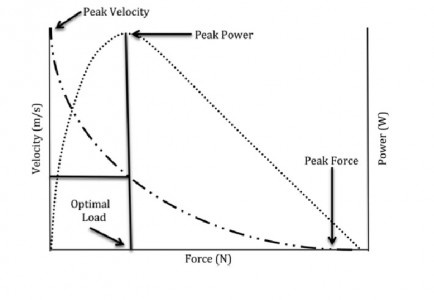
\includegraphics[scale=0.6]{imagenes/OPTIMAL-LOAD-434x300.jpg}
	\caption{Relación entre fuerza y velocidad, punto de máxima potencia 'Optimal Load' o 'Peak Power'.}
	\label{PeakPower}
\end{figure}
\\
\\

La carga seleccionada para el desarrollo óptimo de la potencia suele ser entre el 30-45\% del 1RM, aunque este porcentaje puede variar \cite{Cormie}.

\section{Objetivos}

Los objetivos perseguidos en el desarrollo del proyecto son los siguientes:

\begin{enumerate}
	\item  \textbf{La creación de una aplicación que facilite la labor de un entrenador personal a la hora de realizar, medir y valorar los progresos de un usuario a lo largo del tiempo.} \\
			Probar la viabilidad del desarrollo de una aplicación de salud y deporte utilizando dispositivos de propósito general con sensores, en lugar de un IMU específico.

	\item  \textbf{Investigación de métodos de posicionamiento y rastreo en un escenario real y 3D.} \\
			Realizando la calibración de sensores de bajo coste con el fin de reducir el ruido y el error innato de los sensores.

	\item \textbf{Aplicar los conocimientos adquiridos sobre ingeniería del software.} \\
			Se ha perseguido la aplicación de los conocimientos adquiridos durante el grado en el desarrollo de software en un proyecto real.

	\item  \textbf{Elaboración de un prototipo funcional del proyecto.} \\
			Se persigue la implementación de una aplicación funcional, una aplicación que será instalada en el smartwatch, que provea de los datos y mediciones de la realización del ejercicio. Y otra aplicación instalada en el smartphone que se encargará de recopilar los datos, procesarlos y mostrarlos.
\end{enumerate}

\section{Estructura}

Este documento se encuentra dividido en ocho capítulos. Los cuales desarrollan:

\begin{enumerate}
	\item \textbf{Capítulo 1: Introducción.} Es el capítulo en el que se encuentra esta sección, está formado por tres secciones. La primera llamada Motivación 1.1 describe que es un entrenamiento basado en potencia y los beneficios que se obtiene de este tipo de entrenamiento. La segunda sección denominada Objetivos 1.2, contiene un resumen de los objetivos que se pretenden alcanzar con el desarrollo de este proyecto. La última sección denominada Estructura 1.3, presenta la estructura de los capítulos del presente documento así como una breve descripción de sus contenidos.
	\item \textbf{Capítulo 2: Estado del arte} Este capítulo se organiza en tres apartados. El primero, llamado Estado del mercado 2.1 define el estado actual del mercado de tecnologías que permiten realizar mediciones de entrenamientos basados en potencia. El segundo capítulo denominado Tecnologías 2.2 contiene una breve descripción de las tecnologías que nos van a permitir el desarrollo de este proyecto. Por último la sección llamada Sensores de movimiento en Android 2.3 trata sobre los principales tipos de sensores relacionados con el movimiento que se encuentran disponibles en Android.
	\item \textbf{Capítulo 3: Especificación de requisitos} En este capítulo encontramos los distintos tipos de requisitos que debe cumplir el sistema. Se encuentra estructurado en tres secciones. Requisitos funcionales 3.1, los cuales definen funciones del sistema. En la segunda sección encontramos los Requisitos no funcionales 3.2, los cuales contienen restricciones del sistema relacionadas con el diseño o la implementación. Finalmente, encontramos la sección Requisitos de información 3.3, los cuales hacen referencia a información que debe ser almacenada en el sistema.
	\item \textbf{Capítulo 4: Planificación} Este capítulo se organiza en dos apartados. El primero llamado Planificación 4.1, contiene la planificación general del proyecto, haciendo uso de metodologías ágiles. El segundo apartado denominado Coste del proyecto 4.2, contiene un escueto presupuesto sobre el desarrollo del proyecto.
	\item \textbf{Capítulo 5: Análisis de los datos} Este capítulo está formado por 5 secciones. La primera denominada Introducción al problema 5.1, nos habla sobre porque es importante tratar los datos de los sensores en el desarrollo de este proyecto. La segunda sección llamada Cálculo de la velocidad 5.2, describe como se obtiene la velocidad a partir de la aceleración. La tercera sección denominada Calibración de los sensores 5.3, comenta tres técnicas diferentes para conseguir eliminar la componente gravitacional de la aceleración. La sección Pruebas de calibración 5.4, pone las técnicas descritas en el apartado anterior a prueba. Finalmente, la sección Eliminación de ruido mecánico 5.5, describe un método para eliminar parcialmente el ruido mecánico de los sensores.
	\item \textbf{Capítulo 6: Diseño} En este capítulo se encuentran 5 secciones. La primera, Diseño del sistema 6.1, describe la arquitectura general del sistema. La segunda, Diagrama de clases de la aplicación móvil 6.2, describe atributos, métodos y relaciones de la aplicación móvil. La tercera, Diagrama de clases de la aplicación wear 6.3, describe atributos, métodos y relaciones de la aplicación wear. La cuarta sección denominada Casos de uso 6.4, contiene los distintos casos de uso de los usuarios en el sistema. Finalmente, la sección Diseño de la base de datos 6.5, describe la estructura de la base de datos.
	\item \textbf{Capítulo 7: Implementación} Formado por 3 secciones. La primera llamada Hito 1: Asistente entrenamiento potencia 7.1, describe los pasos realizados para implementar el asistente de entrenamiento. La segunda, denominada Hito 2: Uso del servidor, describe los pasos realizados para implementar la conexión con el servidor. Finalmente, la sección Capturas 7.3, contiene capturas sobre la aplicación.
	\item \textbf{Capítulo 8: Conclusiones y trabajo futuro} Realiza un análisis sobre los objetivos buscados, conseguidos y los resultados del proyecto. Además de exponer cual será el trabajo futuro.
\end{enumerate}

\chapter{Estado del arte}

\section{Estado del mercado}

Existen tres herramientas principales a la hora de monitorizar un entrenamiento basado en potencia:

\subsubsection*{Encoder Lineal}

Un encoder lineal es un dinamómetro que, aplicado al deporte, se utiliza para realizar una medición directa y contínua del espacio recorrido y el tiempo de movimiento de una carga conocida. Pudiendo utilizarse así para calcular la potencia, fuerza o velocidad \cite{encoder}.
\\
\\
Son muy fiables y precisos, pero presentan también algunos inconvenientes. El principal inconveniente es su precio, que puede ser realmente elevado. Por lo su venta no va dirigida a usuarios particulares, si no a profesionales. Además requere de personal cualificado para su uso e interpretación.

\subsubsection*{Push Band}

Push Band es un dispositivo wearable IMU, que conectado a una aplicación permite la monitorización del entrenamiento. Además, dispone de una interfaz web, accesible desde cualquier plataforma\cite{push}.
\\
\\
Si bien su coste no es tan elevado, también presenta inconvenientes. El principal de ellos es que está disponible solo para iOS.

\subsubsection*{Beast Sensor}

Beast Sensor es también un dispositivo wearable IMU, que se conecta a través de una aplicación móvil (disponible en iOS y Android) y es usada para monitorizar el ejercicio\cite{beast}. Además también presenta una interfaz web donde se puede consultar la información de una cuenta.
\\
\\
Las diferencias entre Beast Sensor y Push Band son mínimas, su principal diferencia es que Beast funciona en Android mientras que Push no. Se debe destacar que, tanto estas dos herramientas como los encoders lineales hacen uso de dispositivos de propósito específico, que el usuario debe adquirir expresamente si desea monitorizar su entrenamiento.
\\
Por ello surge este proyecto, con el fin de poder realizar la monitorización del entrenamiento con un dispositivo de propósito general. Como son los smartwatches con Android Wear.


\section{Tecnologías}

\subsection{Android}

Android es un sistema operativo móvil desarrollado por Google y basado en el kernel de Linux, diseñado principalmente para dispositivos móviles y otros dispositivos de pantalla táctil, como smartphones, smartwatches y tabletas. Originalmente fue desarrollado por Android Inc. , la cual fué posteriormente adquirida por Google. Android es además un sistema multiplataforma, lo cual lo ha hecho adquirir el gran éxito y popularidad de la que goza hoy en día.

\subsubsection{Arquitectura de Android}

\begin{figure}[H]
	\centering
	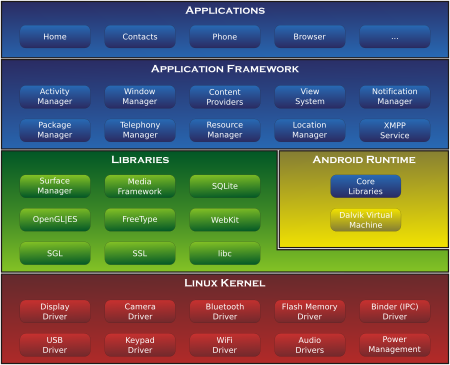
\includegraphics[scale=0.7]{imagenes/capasandroid.png}
	\caption{Arquitectura del SO Android}
	\label{Arquitectura del SO Android}
\end{figure}
\noindent
La arquitectura de Android se encuentra formada por capas. Como podemos apreciar en la figura superior, en la base de la pila se encuentra el kernel de Linux. Construido en C principalmente, es el encargado de la gestión de la memoria, servicios de seguridad y de dar soporte a los controladores.
\\
\\
La capa inmediatamente superior, es la capa del framework de aplicación, la cual incluye librerias y la denominada 'Android Runtime'.
\\
Las librerías son nativas, escritas en C y precompiladas. Entre ellas se destacan:
\begin{itemize}
\item SSL: Proporciona servicios de seguridad y encriptación.
\item SQLite: Motor de bases de datos relacionales.
\item WebKit: Ofrece soporte para el navegador web y su vista webview.
\end{itemize}
\\
\\
El entorno de ejecución o 'Android Runtime' , basado en la máquina virtual de Java, recibe el nombre de Dalvik. La máquina virtual será la encargada de compilar y ejecutar de forma nativa fragmentos de código denominados tazas de código, cada vez que una aplicación es lanzada. Optimizando de esta manera los recursos del sistema y delegando al kernel el threading y el manejo de memoria a bajo nivel.
\\
\\
En la capa inmediatamente superior encontramos el marco de aplicación o 'Application Framework', el cual ofrece una plataforma a las aplicaciones, incluyendo librerías Java. Entre ellas, las más importantes son:
\begin{itemize}
\item Activity Manager. Manejador destinado al ciclo de vida de las actividades.
\item Views. Conjunto de vistas.
\item Location Manager. Proporciona servicios de localización a aplicaciones.
\item Content Provider. Concede accesos a datos de otras aplicaciones.
\item Notification Manager. Facilita el soporte para mostrar notificaciones a las distintas actividades.
\end{itemize}
\\
En la capa superior de abstracción, encontramos la placa de aplicación. La cual engloba a todas las aplicaciones que se encuentren instaladas en el dispositivo.
\\
\subsubsection{Tareas y pila de actividades}

Una aplicación generalmente esta formada por una serie de actividades, las cuales son necesarias para el correcto funcionamiento de la aplicación. Por norma general, cada actividad debe estar diseñada en torno a una clase de acción que puede realizar el usuario y se deben poder comunicar con otras actividades, creándolas y enviando información entre ellas. Pudiendo incluso darse el caso de que una actividad inicie una actividad existente en otra aplicación del dispositivo, lo cual otorga una gran versatilidad.
\\
\\
Podemos definir una tarea como la colección de actividades cuyo objetivo o finalidad es común. Dichas actividades son organizadas en la pila de actividades, la cual se va rellenando en el orden en el que se abre cada actividad.
\begin{figure}[H]
	\centering
	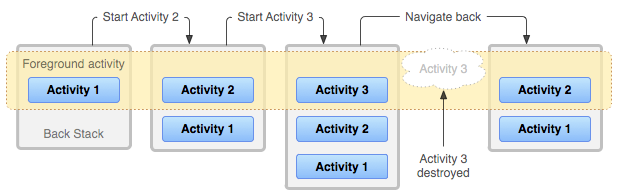
\includegraphics[width=\textwidth]{imagenes/activityStack.png}
	\caption{Pila de actividades de Android.}
	\label{Pila de avtividades}
\end{figure}
\\
\\
En la figura anterior, podemos ver el contenido de la pila en base a diferentes acciones. Cuando creamos una nueva actividad, la actividad anterior sigue mantenida en la pila de actividades, ocupando así la nueva actividad creada la cima de la pila. Al pulsar el botón hacia atrás o destruir una actividad, la actividad que ocupaba la segunda posición en la pila, queda en el tope de la pila y se vuelve a mostrar dicha actividad, liberando los recursos que estaba consumiendo la actividad anterior.
\\
Cuando la pila de actividades se encuentra vacía, la tarea deja de existir y sus recursos son liberados totalmente. Además, si cambiamos a otra actividad de otra aplicación o volvemos a la pantalla de inicio, las actividades de la pila pasaran a segundo plano, deteniéndose, pero la pila de retroceso permanecerá intacta.
%************************************************
\subsection{Android Wear}

Android Wear es una versión del sistema operativo de Google, Android. Desarrollado para usarse como sistema operativo en smartwatches. El sistema operativo fue lanzado por Google en 2014 y puede ser conectado con dispositivos Android a partir de su versión 4.3 o en iPhone a partir de iOS 9. Siendo posible que la funcionalidad varíe en función de la plataforma y versión del sistema operativo.
\\
\\
Actualmente se encuentra en la versión 2.0 en la cual se da mayor independencia al dispositivo wear con respecto al smartphone. Otorgandole así mayor autonomía.
\\
La mayor diferencia entre el ecosistema Android y Android Wear se aprecia en las actividades, tienen un conjunto diferente de eventos que se asocian con el sistema operativo, los más destacados son:
\begin{itemize}
\item Cuando cambia la hora.
\item Cuando llega una notificación.
\item Cuando la intensidad del brillo de la pantalla cambia.
\end{itemize}

\subsection{GoogleAPIClient}
La clase GoogleApiClient es el punto de enlace para los servicios de integración de Google Play (\textit{Google Play Services}). Es decir, cualquier aplicación que quiera hacer uso de alguna API de los servicios de Google, deberá instanciar un cliente de dicha clase en la aplicación.
\\
\\
La clase dispone de una gran multitud de métodos. Algunos requieren que el el cliente GoogleApiClient este conectado, otros se encolan cuando no hay una conexión establecida. Pero para poder ejecutar cualquier operación, debe existir una conexión\cite{GoogleApiClient}.
\subsection{DataAPI}

Es una Api que forma parte de los servicios de \textit{Google Play Services}, los cuales proveen a las aplicaciones de un canal de comunicación adicional, en este caso, para un dispositivo wearable.
La Api Data Layer consiste en una serie de objetos que pueden ser utilizados para enviar y sincronizar datos, en conjunto con los \textit{'listeners'}, para establecer una comunicación.
En nuestro caso vamos a utilizar la Api para establecer un canal de comunicación entre el dispositivo Wearable y el móvil construido sobre el estándar Bluetooth \cite{DataAPI}.

\begin{figure}[H]
	\centering
	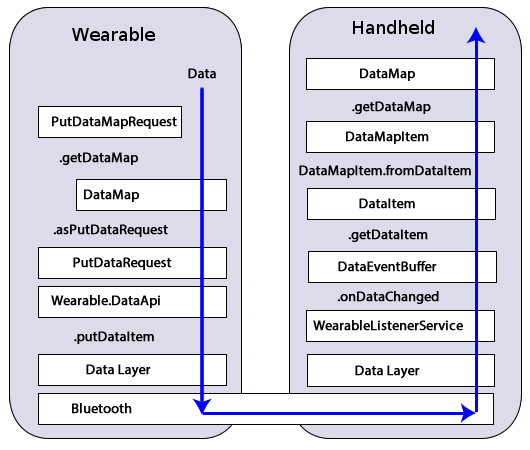
\includegraphics[scale=0.5]{imagenes/dataApi.png}
	\caption{Estructura de la capa DataApi.}
	\label{DataApi}
\end{figure}
\noindent
Para emplear esta API, se debe disponer de una versión de Android igual o superior a la 4.3 (API 18) en el dispositivo wear. La primera versión disponible de Android Wear está basado en Android 4.4.2 KitKat (API 19), por lo que es compatible con todos los dispositivos Android Wear. Además, cabe destacar que se debe de utilizar la última versión de Google Play services \cite{playServices}.


\subsection{Firebase}

Firebase \cite{firebase} es una aplicación web y móvil del tipo BaaS (Backend-as-a-Service), es decir ofrece funcionalidades propias de un servidor por medio de una interfaz. Permitiendo a las aplicaciones conectarse y sincronizarse con un servidor de una manera rápida y sencilla sin necesidad de implementar una API Rest.
\\
\\
En su esencia, es principalmente una base de datos en tiempo real, la cual hace uso del protocolo WebSockets en lugar de HTTP. Y su principal ventaja es que todos los clientes de la aplicación en tiempo real sincronizan sus datos, de manera que todos los clientes de la base de datos los reciben de manera instantánea.
\\
Utiliza un modelo de base de datos NoSQL. Los datos se almacenan en formato JSON. Y como tal ofrece diferentes funcionalidades en comparación con una base de datos relacional, siendo la velocidad su mayor ventaja.
\\
\\
Además de brindar una base de datos, provee una amplia lista de funcionalidades , sus principales son:
\begin{itemize}
\item Almacenamiento de archivos. Permite almacenar archivos en '\textit{Google Cloud Storage}' de forma directa desde el cliente.
\item Autenticación. Ofrece un sistema de autenticación por medio de email/contraseña, además soporta autenticación en base a '\textit{OAuth2}' con multitud de servicios, como Google, Facebook, Twitter y Github.
\item Servicio de alojamiento. Permite almacenar y servir archivos estáticos utilizando el protocolo HTTP/2.
\end{itemize}


\subsection{Sensores}

Se define como sensor a un elemento o dispositivo electrónico, que detecta eventos o cambios en el entorno en el que se encuentran y envían la información de dicho evento a otro dispositivo electrónico.
\\
\\
La sensibilidad es definida como el ratio entre la señal de salida y la magnitud de la propiedad medida. La mayoría de sensores tienen una función de transferencia lineal.

\subsubsection{Desviaciones de los sensores}

Los sensores no pueden replicar una función de transferencia ideal. Presentando las diferentes fluctuaciones:

\begin{itemize}
\item El rango de la señal de salida esta limitado, soliendo obedecer normalmente a un Vpp. Por lo que la salida del sensor alcanzará eventualmente un mínimo y un máximo.

\item La sensibilidad práctica difiere del valor especificado. Denominado como error de sensibilidad.

\item Si la señal de salida difiere del valor correcto por una constante y, se dice que el sensor posee un error de \textit{\textbf{offset}} (desplazamiento) o error bias.

\item La no linearidad es la desviación de la función de transferencia de un sensor.

\item La desviación causada por cambios rápidos en la propiedad que se esta midiendo se conoce como error dinámico.

\item Si la señal de salida cambia de manera muy lenta, independientemente de la variación de la propiedad medida, dicho fenómeno es conocido como \textit{\textbf{drift}} (desvío).

\item El ruido es una desviación aleatoria de la señal que varía con respecto al tiempo.

\item Los sensores con una señal de salida digital, la salida es esencialmente una aproximación de la propiedad medida. Dicho fenómeno es llamado error de quantización.

\item Cuando la señal es monitorizada digitalmente, la frecuencia de muestreado puede causar errores dinámicos, o si la entrada de datos cambia periódicamente a otra frecuencia, puede producir errores de \textit{antialising} (acoplo).

\end{itemize}

\section{Sensores de movimiento en Android}

La Api de Android provee de varios sensores con el fin de poder monitorizar el movimiento del dispositivo.
\\
\\
Android provee de sensores basados en software o hardware. Los sensores software como la gravedad, vector de rotación, contador de pasos etc, han de ser implementados usando sensores hardware (acelerómetros, giroscopios y magnetómetros).
\\
Actualmente, la gran mayoría de dispositivos Android tradicionales contienen acelerómetros, giroscopios y magnetómetros. Sin embargo no todos los dipositivos Android Wear disponen de estos tres sensores, siendo el caso más común que dispongan de acelerómetro y giroscopio únicamente \cite{SensorGoogle}.

\subsection{Acelerómetro}

Un acelerómetro es un dispositivo que mide vibración o aceleración propia de una estructura. Siendo la aceleración el ratio del cambio de velocidad con respecto al tiempo.
\\
La fuerza causada por las vibraciones de un cambio en el movimiento (aceleración) causa que la masa mueva el material piezoeléctrico generando una carga que es proporcional a la fuerza que experimenta (Fuerza de la gravedad incluida) .

\begin{figure}[H]
	\centering
	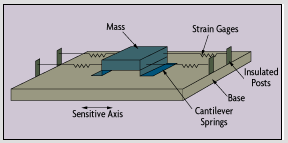
\includegraphics[scale=0.7]{imagenes/piezoelectrico.png}
	\caption{Acelerómetro piezoeléctrico}
	\label{Accelerometer}
\end{figure}
\noindent
Los acelerómetros \textit{multi-axis} (varios ejes) son capaces de detectar magnitudes y direcciones de la propia aceleración como un vector cuantitativo \cite{WikipediaAccelerometer}.


\subsubsection{Acelerómetro en Android}

El acelerómetro mide la aceleración aplicada al dispositivo móvil, incluyendo la fuerza de la gravedad. Siguiendo el estándar de coordenadas que podemos apreciar en la siguiente figura:

\begin{figure}[H]
	\centering
	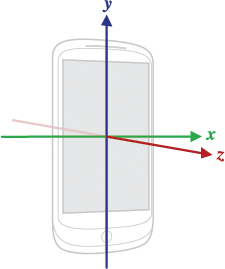
\includegraphics[scale=0.8]{imagenes/axis_device.png}
	\caption{Sistema de coordenadas relativo a la API de los sensores.}
	\label{Sistema de coordenadas sensores}
\end{figure}
\noindent
Es el sensor principal que se debe monitorizar para realizar un seguimiento de movimiento. Puesto que esta presente en todos los dispositivos móviles comerciales y tiene un consumo de energía de hasta 10 veces menor que el resto de sensores.
\noindent
La API provee de una serie diferente de posibilidades para el uso del acelerómetro \cite{GoogleAcel}:

\begin{table}[H]
\centering
    \begin{tabular}{p{5.0cm} p{2.0cm} p{5.0cm} p{2.0cm}}%{|l{2cm}|l|l{2cm}|c|}
    \hline
    Sensor & Estructura de Datos & Descripción & Unidades \\ \hline
    \\ TYPE\_ACCELEROMETER (API 3) & Vector[3] & Fuerza de aceleración a lo largo de los 3 ejes. Incluyendo la gravedad. & m/s\^2 \\\\ \hline
    TYPE\_ACCELEROMETER\\\_UNCALIBRATED (API 26) & Vector[3] & La aceleración medida a lo largo de los 3 ejes sin ningún tipo de desviación bias.  & m/s\^2 \\\\ \hline
    \\TYPE\_GRAVITY (API 9) & Vector[3] & La aceleración producida por la fuerza de la gravedad. & m/s\^2 \\\\ \hline
    TYPE\_LINEAR\\\_ACCELERATION (API 9) & Vector[3] & La aceleración a lo largo de los 3 ejes. Excluyendo la gravedad & m/s\^2 \\\\ \hline
    \end{tabular}
\end{table}

\subsection{Giroscopio}

Un giroscopio es un dispositivo usado para medir el grado de rotación en radianes por segundo a lo largo de un eje de coordenadas. Es decir, son dispositivos que miden la velocidad angular.
\noindent
En los últimos años, ha aumentado el empleo de giroscopios de estructura vibrante en todo tipo de industrias, como móviles, vehículos, fotografía, etcétera.

\subsubsection{Giroscopios de estructura vibrante}

Los giroscopios de estructura vibrante miden la velocidad angular de la fuerza causada por el efecto Coriolis aplicada a un elemento en vibración. Por lo que la precisión de la velocidad angular medida difiere dependiendo del material. En la siguiente figura se puede apreciar la estructura:

\begin{figure}[H]
	\centering
	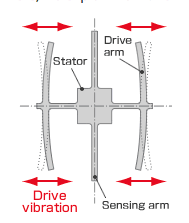
\includegraphics[scale=0.7]{imagenes/gyro.png}
	\caption{Giroscopio de estructura vibrante.}
	\label{Giroscopio de estructura vibrante}
\end{figure}

\subsubsection{Giroscopios en Android}
\\
El giroscopio mide el grado de rotación a lo largo de los 3 ejes de coordenadas del dispositivo, siguiendo el mismo sistema de coordenadas de la API. La rotación es positiva en el sentido anti\-horario.

\begin{table}[H]
\centering
    \begin{tabular}{p{5.0cm} p{2.0cm} p{5.0cm} p{2.0cm}}%{|l{2cm}|l|l{2cm}|l|}
    \hline
    Sensor & Estructura de Datos & Descripción & Unidades \\ \hline
    \\TYPE\_GYROSCOPE (API 3) & Vector[3] & Ratio de rotación 3-axis. & rad/s \\\\ \hline
    TYPE\_GYROSCOPE\\\_UNCALIBRATED (API 18) & Vector[3] & Ratio de rotación 3-axis.Sin compensación drift. & rad/s \\\\ \hline
    TYPE\_ROTATION\_VECTOR (API 9) & Vector[3] & Rotación vector componente a lo largo de los ejes (eje * Sin(O/2)) & Sin unidades \\ \hline
    \end{tabular}
\end{table}
\noindent
Por defecto los giroscopios también proveen de datos sin ningún tipo de filtrado, por lo que la varianza 'bias' y el ruido inherente están presentes en los datos obtenidos. El tipo de sensor \textbf{TYPE\_GYROSCOPE} provee de datos con compensación 'bias'. El tipo de sensor \textbf{TYPE\_GYROSCOPE\_UNCALIBRATED} no provee ningún tipo de calibración, obedeciendo a la siguiente relación para cada eje.
\\

\[calibrated_x ~= uncalibrated_x - bias_estimate_x\]



\subsection{Magnetómetro}

Un magnetómetro es un instrumento cuya finalidad es medir la intensidad de un campo magnético. Pudiendo  dividirse en dos tipos:

\begin{itemize}
\item Magnetómetros escalares. Los cuales miden la fuerza total de los campos magnéticos bajo los que se encuentran. Es decir, miden la sumatoria de la fuerza magnética en todas las direcciones.

\item Magnetómetros vectoriales. Tienen la capacidad de medir la intensidad del campo magnético bajo los que se encuentran en una dirección en concreto.
\end{itemize}

\begin{figure}[H]
	\centering
	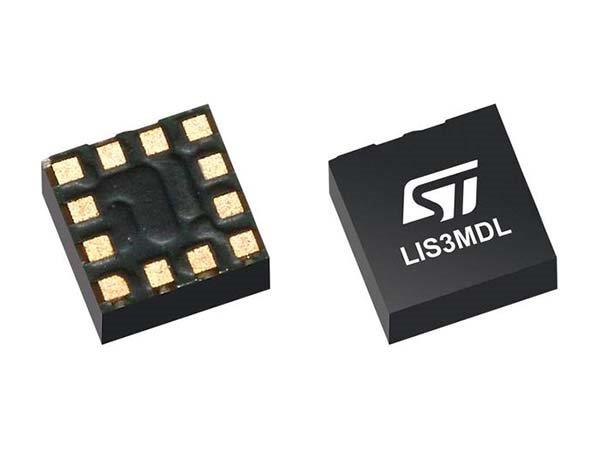
\includegraphics[scale=0.5]{imagenes/magnetometer.jpg}
	\caption{Magnetómetro.}
	\label{Magnetometro}
\end{figure}

\subsubsection{Magnetómetro en Android}

El magnetómetro en Android mide cambios en la intensidad del campo magnético terrestre .

\begin{table}[H]
\centering
    \begin{tabular}{p{5.0cm} p{2.0cm} p{5.0cm} p{2.0cm}}%{|l{2cm}|l|l{2cm}|l|}
    \hline
    Sensor & Estructura de Datos & Descripción & Unidades \\ \hline
    TYPE\_MAGNETIC\\\_FIELD (API 3) & Vector[3] & Campo geomagnético  3-axis. & $\mu$T \\\\ \hline
    TYPE\_MAGNETIC\\\_FIELD\_UNCALIBRATED (API 18) & Vector[6] & Campo geomagnético  3-axis sin calibración de 'Iron'  Estimación bias de 'Iron' 3-axis  & $\mu$T \\ \\ \hline
    \end{tabular}
\end{table}
\noindent
El tipo \textbf{TYPE\_MAGNETIC\_FIELD} es similar es calibrado siguiendo la siguiente regla:

\[calibrated_x ~= uncalibrated_x - bias_estimate_x\]
\noindent
Se debe tener en cuenta que los sensores no calibrados pueden contener desviación bias, pero contienen menos saltos en la frecuencia de muestreo, por lo que dichos sensores proveen datos más frecuentemente y consecuentemente, más fiables en cuanto a frecuencia.
